\documentclass[11pt]{article}
\usepackage[utf8]{inputenc}

\usepackage[margin=2.1cm]{geometry}
\usepackage[utf8]{inputenc}
%\usepackage{dirtytalk}
\usepackage{titling} % multiple title pages
\usepackage[autostyle]{csquotes}
\let\oldenquote\enquote
\renewcommand{\enquote}[1]{{\itshape\oldenquote{#1}}}
\usepackage[T1]{fontenc}
\usepackage{lmodern}

% \usepackage{bookmark}% http://ctan.org/pkg/bookmark

\usepackage{pdfpages}
\usepackage{soul}
\pdfminorversion=7

% \usepackage[hidelinks]{hyperref}
% \hypersetup{
%     colorlinks=blue,
%     linkcolor=blue,
%     filecolor=blue,      
%     urlcolor=blue,
% }


\title{}


\date{}


\makeatletter
\renewcommand\@bibitem[1]{\item\if@filesw \immediate\write\@auxout
    {\string\bibcite{#1}{Exhibit \the\value{\@listctr}}}\fi\ignorespaces}% <------------
\def\@biblabel#1{Exhibit #1:}% <-------------------
\makeatother

\makeatletter
% we use \prefix@<level> only if it is defined
\renewcommand{\@seccntformat}[1]{%
  \ifcsname prefix@#1\endcsname
    \csname prefix@#1\endcsname
  \else
    \csname the#1\endcsname\quad
  \fi}
% define \prefix@section
\newcommand\prefix@section{\underline{Section \thesection: }}
\makeatother


\usepackage{amsmath}
\usepackage{amssymb}
\usepackage[labelfont=bf]{caption}
% \usepackage[nolists]{endfloat}
\usepackage{setspace}\setstretch{1.167} % prerequisite of geometry
% \usepackage[textwidth=17.0cm, lines=42, hcentering]{geometry}
% \usepackage[colorlinks]{hyperref}
\usepackage[utf8]{inputenc}
\usepackage[british, cleanlook]{isodate}
\usepackage[pagewise, modulo, displaymath, mathlines]{lineno}
\usepackage{microtype}
%\usepackage[medfamily, textlf, mathlf]{MyriadPro}\renewcommand{\familydefault}{\sfdefault}
\usepackage[amssymb]{SIunits}
\usepackage[bib, enum, eqno, lineno, toc]{tabfigures}

\usepackage{fancyhdr}
\usepackage{soul}
\usepackage{tikz}
\setlength\parindent{0pt}
\newcommand{\mybullet}{\,\textbullet\,}

\setcounter{tocdepth}{4}
\setcounter{secnumdepth}{4}


\pagestyle{fancy}
\fancyhf{}
%\tikz[remember picture, overlay] \node at (current page.center) {\includegraphics{outline_letterhead}};
\renewcommand{\headrulewidth}{1pt}

\lhead{EB-2 NIW Permanent Residence Petition for Mr. Xxx Xxx}
% \rhead{\thepage}
\cfoot{\thepage}




\begin{document}
\newcommand{\tc}[1]{\textcolor{blue}{#1}}

\vspace*{10em}

%\vfill*{}

%\tc{Attach checks with clipper. See check writing instructions: https://www.uscis.gov/forms/filing-fees}

%\begin{figure}
%\includegraphics[width=0.8\textwidth]{aux/check.jpeg}
%\end{figure}

%\vspace*{5em}

\begin{center}
 \Large{\textbf{Immigrant Petition for Alien Worker
for the Alien with Exceptional Ability in Science (EB2-NIW)}}
\end{center}


\vspace*{1em}

\begin{center}
\Large{\textbf{TABLE OF CONTENTS}} 
\end{center}


\begin{enumerate}
 \item Form G-1145 e-Notification of Application/Petition Acceptance
 \item Form I-140, Immigrant Petition for Alien Worker, with \$700 filing fee
 \item Form I-907, Request for Premium Processing Service, with the \$2,805 filing fee
 \item Form ETA-9089
 \item Photocopies of the passport, H1B visa, Form I-797, Form I-94.
 \item Initial Evidence in Support of the I-140 Immigrant Petition
 \item Statement from Mr. Xxx LastName detailing plans on how he intends to continue work in the United States
 \item List of Exhibits
 \item Exhibits 1--23
\end{enumerate}


\pagebreak

% \renewcommand\href[3][\relax]{#3}

% \maketitle

\sloppy

% \section{Introduction}

\vspace{4em}


\begin{center}
 \Large{\textbf{Initial Evidence in Support of the I-140 Immigrant Petition}}
\end{center}

\vspace{4em}


\begin{tabular}{ll}
\textbf{Petitioner and Beneficiary:} & Xxx LastName\\
\textbf{Classification Sought:} & Employment-Based Immigration, Second Preference\\
& Exceptional Ability in Science \\
& with a “national interest waiver” of the job offer (EB2-NIW).\\
& Sec. 203(b)(2)(B) INA [8 U.S.C. 1153].\\
\end{tabular}

\vspace{2em}


To whom it may concern,

\vspace{2em}



\newcommand{\fie}{Machine Learning}
\newcommand{\dr}{Mr. LastName }
\newcommand{\drs}{Mr. LastName's }

%\newcommand{\qu}[1]{\say{\emph{#1}}}


\newcommand{\referrerA}{(Name, Title, Institution\\}
\newcommand{\referrerB}{(Name, Title, Institution\\}



This initial evidence is the attachment to Mr. Xxx LastName’s I-140 Immigrant Petition for Alien Worker. This evidence shows that Mr. LastName is an alien of exceptional ability in the sciences, specifically in \underline{\fie{}}, who will substantially benefit the national economy, educational interests, and welfare of the United States \textit{(Sections \ref{section1} and \ref{section2})}. \\


\dr satisfies \underline{four} of ten criteria listed in 8
CFR, Section 204.5(k)(3)(ii), namely:
\begin{enumerate}
    \item Evidence that dr holds an advanced degree in Xxxx from a prestigious university. \textit{(Section \ref{degree})}

    \item Letters from current or former employers documenting \drs xx years of full-time experience in the \fie{} field. \textit{(Section \ref{yoe})}

    \item Evidence that \dr has commanded a high salary for services that demonstrates his exceptional ability. \textit{(Section \ref{compensation})}
    
    \item Evidence of recognition of \drs achievements and significant contributions to the field by business organizations and his peers, including authorship of scholarly articles and patents in the field. \textit{(Section \ref{conference} \ref{industry} \ref{honor} \ref{papers} \ref{patents})}
\end{enumerate}

\dr requests a national interest waiver of the job offer pursuant to Section 203(b)(2)(B)(i) of the Act because he satisfies all three criteria for such a waiver described in \textit{Matter of Dhanasar},26 I\&N Dec. 884 (AAO 2016), namely:

\begin{enumerate}
\item \drs proposed work in \fie{} has both substantial merit and national importance. \textit{(Section \ref{section2})}

\item \dr is well-position to advance the proposed endeavor due to his exceptional abilities and expertise. \textit{(Section \ref{section1})}

\item On balance, it would be beneficial to the United States to waive the job offer and labor certification requirements for \dr. \textit{(Section 3, and Statement from Mr. Xxx LastName detailing plans on how he intends to continue work in the United States)}

\end{enumerate}

In the United States, \dr plans to continue work in the area of expertise. \textit{(Please refer to the Statement from Mr. Xxx LastName detailing plans on how he intends to continue work in the United States and to Exhibit 14, his current job offer.)} \\

Pursuant to 8 CFR, Section 204.5(k)(1), \dr may file a petition on Form I-140 for classification under Section 203(b)(2) of the Act as an alien of exceptional ability in the sciences on his own behalf because he is seeking an exemption from the requirement of a job offer in the United States pursuant to Section 203(b)(2)(B) of the Act.


\pagebreak




\section{\dr is an alien of exceptional ability in \fie{}, who will substantially benefit prospectively the national economy, educational interests, and welfare of the United States.}
\label{section1}

\subsection{ \dr is an expert in the field of \fie{} with Xxx years of application experience in the industry of proposed employment.}
\label{yoe}

After \dr obtained his Xxx’s degree, he engaged in \fie{} research and application development. In the past Xxx years from Xxx to now, he has served Xxx companies. His work experience mainly focuses on the research and application of \fie{} in the recommendation field. \cite{workexp}. The following are the details: 


\begin{itemize}
    \item Four years at Xxx as a Xxx, from Apr Xxx to the present. His main research and work domain was to optimize Xxx video recommendation products, research cutting-edge recommendation technology, and apply them to solve Xxx movie recommendation problems, thus improving user experience, including improving the international user experience on Xxx TV, modeling the long-term user engagement, offline evaluation, list-wise learning, etc.

    \item One year at Xxx as the Xxx, from Jun Xxx to Apr Xxx, leading the algorithm team of Xxx's advertising recommendations; my responsibilities were mainly to optimize product recommendations on the Suning e-commerce shopping platform and improve user shopping experience. Specific contents include auto bidding, smart budget pacing, product recommendation, CTR/CVR improvement, etc.
\end{itemize}


\subsection{\dr has received degrees including the Master degree in Xxx from high-ranking universities.}
\label{degree}


\dr obtained his Bachelor of Science Degree from Xxx. The Science Diploma of \dr has been translated into English, along with the certificate of accuracy of the translation. \cite{bachelor} \\


In April Xxx, \dr defended and submitted his Master's dissertation. xxx \\

According to the US. News University Ranking 2023, it is the 18th best university in China and one of the Top Xxx universities in the world, and it's the xxxth best university in the world in the Mathematics field. \cite{schoolrank} \cite{schoolrank2}



\subsection{\dr have commanded a salary for services that demonstrates his exceptional ability}
\label{compensation}


%\begin{figure}[h!]
%\centering
%\includegraphics[width=0.5\textwidth]{salary/local_wage.png}
%\end{figure}

O*Net Online is an independent third-party organization that provides authoritative regional industry salary levels. According to data from O*Net regarding local wages in the Bay Area for Software Engineer, \drs compensation falls within the top 10\%, indicating high recognition for his work in the market. \cite{onetwage} \\


\subsection{Other industry employees recognize \drs exceptional knowledge of \fie{} and consider \dr a top expert in the field.}
\label{conference}

\dr is actively in the industrial form and has given speeches at several public events; in 2020, \dr initiated the XxxRecommendation\&Advertisement Tech Summit and had about 100 audiences, and most came from the \fie{} participation from tech companies where he got a lot of reputations from. Suning's official website reported this event. \cite{summit} \\

\drs global recognition is evident from the support letter written by one of the beneficiaries who never worked with \dr. \cite{rl_referrer1} \\


\enquote{Mr. LastName gave a fascinating talk about Xxx, Xxxx, and recommendation systems that impressed the audience, including me. \ul{His proposal of Xxx, which is really helpful for solving the Xxx recommendation problems.}} \referrerA


\enquote{Mr. LastName explores advanced technologies and applying them across various industries. \ul{His ability to connect academia and industry is crucial, fostering collaboration and international benefit-sharing, surpassing the impact of academic-to-commercial institutions connections.}} \referrerA


\enquote{He actively engaged in industry conferences and tech forums, exchanging ideas with leading firms like Alibaba, JD.com, Microsoft, and Tencent to stay abreast of industry trends and promote technological advancements in recommendation systems.} \referrerA


\subsection{ \dr has performed in a critical role in the commercial company and earns great honors he deserves.}
\label{honor}

During \drs tenure as a Senior \fie{} Engineer and Tech Lead at Xxx, Mr. LastName demonstrated exceptional performance, resulting in significant economic gains for the company. He received numerous awards for his contributions, including the \ul{prestigious 2017 Outstanding Employee for his endeavor in recommendation algorithm technology}. Additionally, he led his team to outstanding performance, earning the \ul{2018 Excellent Team Award} among numerous competing teams. \cite{honor} \\


\enquote{Mr. LastName received several awards from Xxx, including the 2017 Best Employee Award for his outstanding contribution to the recommendation algorithm. This prestigious award, bestowed upon only 10 individuals out of 2,000 employees annually, signifies his exceptional commercial impact, outstanding performance, and influence within the company. The recognition from senior management underscores Mr. LastName's remarkable achievements.} \referrerA

Currently, \dr is working for a US company based in San Francisco, and his co-workers shows his well-positioned. \\


\enquote{His innovative approach to optimizing the entire homepage, rather than individual videos and other works, \ul{improves the homepage user experience, positioning Xxx as a leader in the AVOD field. His outstanding performance puts him far beyond other team members.}} \referrerA


\subsection{ \dr has couple publications in the fields of \fie{}.}
\label{papers}

\dr has published four peer-reviewed papers with two as a first author and two as a second author, both in \fie{} field, and got nine citations total(since the citations are in Chinese, Google Scholar does not have an index). Although the publication is not a very high impact factor of the journals, \dr still gets a good reputation from the reviewers. \cite{papers} \\

\enquote{His thesis left a strong impression on me and proved beneficial to my own research. \ul{Mr. LastName's paper addresses the challenge of embedding scale in deep learning models, a crucial aspect of machine learning.} For instance, famous brands like LV and Wellington steak have attributes at different scales. } \referrerA


\subsection{ \dr has three patents published, and those patents help Xxx build up moat. }
\label{patents}

\dr is actively involved in researching and applying \fie{} at Xxx. Apart from contributing to the company's economic growth, \dr has also obtained three invention patents based on his research archivement, one of them as a first author and two as a second author, which strengthens the company's patent portfolio. All three patents are about leveraging \fie{} technology to optimize advertisement recommendation systems with innovation methods; those patented innovations are widely acknowledged and respected within the industry, evidenced by 24 citations. \cite{patents} \\

The patent \textit{\ul{The method and system launched based on advertising creative optimization advertisement}} issued by \dr as the first author proposes a machine learning algorithm to solve the global optimization problem of different recommendation targets. \ul{It has been cited 20 times by top companies in the advertising recommendation field, including Beijing Focus, Tencent, Alibaba, and Bank of China, etc}, and the following chart shows the citations of this patent provide by Google Patent. \cite{patents} \\



\begin{figure}[h!]
\centering
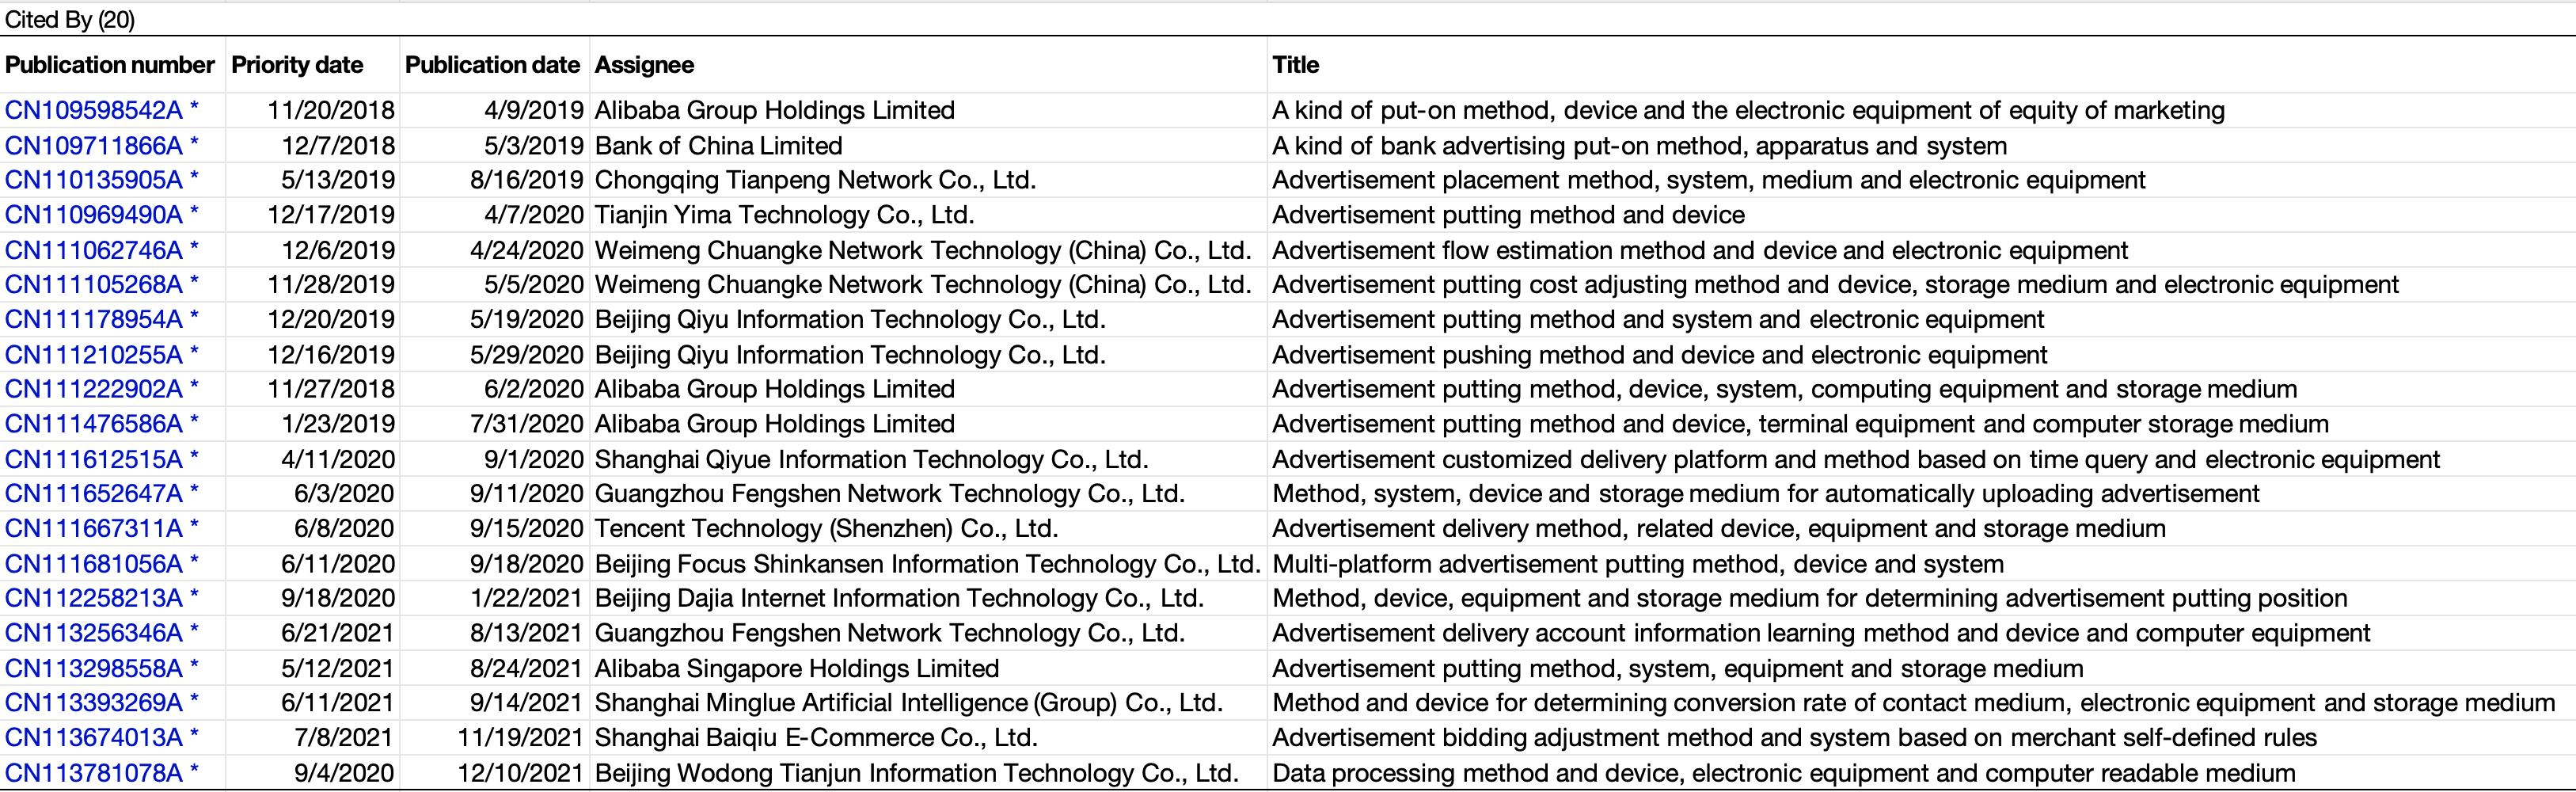
\includegraphics[width=1.0\textwidth]{papers/patent_cites2.png}
\end{figure}


\enquote{Mr. LastName also published three patents in advertising recommendation, which enhanced the company's technical capabilities and established competitive advantages. These patents demonstrate Mr. LastName's strong innovation prowess and his ability to contribute meaningfully to technological advancements.} \referrerA



\pagebreak


\section{\drs proposed employment has both substantial merit and national importance for the United States.}
\label{section2}

\subsection{ \fie{} is an area of substantial merit and national importance for the United States. }
\label{section21}

\enquote{AI is a top priority for President Biden, and the Biden-Harris Administration is taking important steps to promote the safe, secure, and trustworthy use of AI.} (by \ul{https://ai.gov/actions/} from WHITEHOUSE) \\

October 2023, president Joe Biden signed an executive order \textbf{Executive Order on the Safe, Secure, and Trustworthy Development and Use of Artificial Intelligence}, and it says:

\enquote{Review and initiate any policy changes the Secretary determines necessary and appropriate to clarify and modernize immigration pathways for experts in AI and other critical and emerging technologies, including O-1A and EB-1 noncitizens of extraordinary ability; EB-2 advanced-degree holders and noncitizens of exceptional ability; and startup founders in AI and other critical and emerging technologies using the International Entrepreneur Rule;} \\

\fie{} is the most important branch of artificial intelligence(AI); in the WHITEHOUSE file NATIONAL ARTIFICIAL INTELLIGENCE RESEARCH AND DEVELOPMENT STRATEGIC PLAN 2023 UPDATE, \textbf{it mentioned ML(Machine Learning) over 15 times}, and \dr intends to work in the field of \fie{} in the following decades, which will make a great contribution to the states benefits. \\

\enquote{The Biden-Harris Administration is committed to advancing responsible AI systems that are ethical,
trustworthy, and safe, and serve the public good. The fiscal year (FY) 2023 President’s Budget Request
included substantial and specific funding requests for AI R\&D, as part of a broad expansion of federally
funded R\&D to advance key technologies and address societal challenges. The CHIPS and Science Act of
20227 and Consolidated Appropriations Act, 20238 reflect Administration and Congressional support for
an expansion of federally funded R\&D, including AI R\&D.} (from the NATIONAL ARTIFICIAL INTELLIGENCE RESEARCH AND DEVELOPMENT STRATEGIC PLAN 2023 UPDATE) \\


\subsection{ \drs work in \fie{} is substantial merit and will be beneficial to the United States. }
\label{section22}

\drs work is substantial merit and his contributes significantly benefits the national interests of the United States, as evidenced by the following points:


\begin{itemize}
    \item \dr contributed a lot to the open-source community, where his projects have already benefited American companies to create more career positions. His ongoing success will further enhance the prospects for numerous companies, and more important his efforts in the open-source community will allow the United States to maintain its technological edge in \fie{}.

    \item \drs participation in industry forums is pivotal in advancing machine learning technology. By doing so, he contributes to maintaining the United States' technological leadership in artificial intelligence(AI).
    
    \item \drs exceptional performance in his current employment at Xxx Inc. is reflected in his high compensation, which helps Xxx Inc.
\end{itemize}

\enquote{Mr. LastName's pivotal contributions during his x-year tenure at Xxx have been instrumental in the company's success, \ul{helping the company build market dominance in Australia, Canada, Central and South America, and the United Kingdom.}} \referrerA

\enquote{Mr. LastName's proficiency in Machine Learning, particularly recommendation algorithms, has profoundly helps our company. His project holds immense practical value for businesses in our sector, particularly small and medium-sized enterprises like us. } \referrerA


\enquote{Mr. LastName explores advanced technologies and applying them across various industries. \ul{His ability to connect academia and industry is crucial, fostering collaboration and international benefit-sharing, surpassing the impact of academic-to-commercial institutions connections.}} \referrerA


\enquote{His involvement in industry events helps to advance Machine Learning technology across various companies, which is beneficial for all companies and contributes to the country's economy.} \referrerA


\enquote{Mr. LastName actively contributes to the open-source community and participates in industrial forms, offering valuable codes that benefit both individuals and businesses, especially startup like us. \ul{His endeavors contribute to technological advancements and ensure the competitiveness of commercial products.}} \referrerA


\enquote{Mr. LastName's contributions can provide US companies with a competitive edge over international rivals. By leveraging his expertise, American enterprises can adopt advanced AI technologies to enhance productivity, thus supporting US economic vitality and global competitiveness.} \referrerA



\pagebreak

\section{On balance, it would be beneficial to the United States to waive the job offer and labor certification requirements for \dr }


\enquote{The purpose of the labor certification process (PERM Labor Certification) is to assess whether a candidate meets minimum competency standards. However, this standard evaluation can’t capture Mr. LastName's substantial contributions and their broader impact. \ul{His achievements far exceed the minimum requirements outlined by PERM. Therefore, exempting Mr. LastName from the PERM process will not adversely affect the US labor market. Instead, his work in academia and industry will elevate the overall technical proficiency of the US talent pool, enhance labor skills, and improve labor welfare benefits.}} \referrerA

\enquote{While the standard EB2 process necessitates approval via a labor certification from the Department of Labor, \ul{try finding U.S. workers meeting the minimum competency standards is only a baseline, and this baseline is inappropriate for technology talent, particularly for Machine Learning and Artificial Intelligence participators.} Exceptional engineers like Mr. LastName can often surpass the impact of an entire team, bringing tangible economic benefits to enterprises, especially small and medium-sized ones like ours. } \referrerA


\enquote{Given his exceptional qualifications, I believe it's appropriate to exempt him from PERM. This benefits the United States by enhancing its employment environment and improving welfare benefits for American technology professionals.} \referrerA

\enquote{\ul{Mr. LastName's exceptional work as a machine learning engineer has significantly bolstered Xxx's leadership in the AVOD sector.} Waiving the PERM to such exemplary professionals serves the national interests of the United States and will not hurt the US labor market.} \referrerA



In conclusion, the initial evidence presented in Sections 1 and 2 and in the attached Exhibits shows that \dr has a degree of expertise significantly above that ordinarily encountered in \fie{}. \\

\dr is a well-recognized expert in the industrial and scientific field of \fie{}. He will continue working in the field of his expertise in the United States. Supporting letters from experts in the field state that \drs activity in industrial form and open-source community would benefit the United States in industrial, academic, and environmental applications. \\


Because of his record of successful achievement in the area of national importance, \dr offers contributions of such value that, on balance, they would benefit the United States even assuming that other qualified U.S. workers are available. The requirement of the lengthy process of obtaining the labor certification would interrupt and delay the work being performed by \dr and would have a negative impact on the national interests of the United States.
Thus, \dr fully satisfies all requirements and regulations listed in INA Section 203(b)(2) and I ask the reviewer to approve \drs petition for the permanent residence under the category of an alien of exceptional ability with the national interest waiver. \\



Please contact me at the following address for any additional evidence.\\

Yours faithfully, \\


\vspace{4em}
Xxx LastName\\

Address: \\
Tel: +1 xxx-xxx-xxxx\\
Email: xxx\\



\newpage



\subsection*{Statement from Mr. Xxx LastName detailing plans on how he intends to continue work in the United States}

\today\\


My name is Xxx LastName, the recipient of the I-140 Immigrant Petition for Alien Worker, seeking EB2-NIW immigrant classification based on exceptional ability in \fie{}. With over a decade of dedicated service in the technology industry, I have contributed significantly to top-tier tech companies over the world. I have influenced numerous professionals across various companies through active engagement in industry forums and impactful presentations. Furthermore, startups and leading tech corporations have widely embraced my open-source projects. Additionally, my publications of papers and patents have helped fortify the nation's and companies' competitive advantages. \\


Currently I reside in the Bay Area work for Xxx Inc, as a Xxx at Xxx, I contribute to delivering top-tier streaming video experience to our users, and my mainly work is leverage \fie{} technology to improve user's homescreen movie recommendation result. With extensive expertise in the fields of \fie{} and Artificial Intelligence, I aim to further my research and development endeavors in these domains within the United States. \\


If I can get a permanent residence permit in the United States, it can help me easily do the research and development for the state, and Silicon Valley has many meetups around technology, I could be more actively engage these meetups, share what I've learned, and push industrial technology development. Also, being in the United States would let me be more involved in the open-source community cause it will make it easier to work with others in the open-source community and learn more about their pain points, thus iterating the open-source problem and helping more people, thus keep US advance in AI. But without a permanent residence permit, these things would be harder to do. \\ 


My research and work plan in the next two years is to focus on three aspects:
\begin{enumerate}
    \item Participate in technical conferences and entrepreneurial conferences in the field of \fie{} and AI, know more technical peers, and conduct technical exchanges with them. In November Xxx, I participated in the AI conference initiated by Sky9 Venture Capital, held by many AI Founders(LanceDB Founder, MindsDB Founder, etc.), technicians, and capital investors have collided with them and come up with many entrepreneurial ideas and plans, which shows that I am actively participating in exchanges in the AI field in the United States. \cite{ai_happy_hour}

    \item In terms of serving at Xxx, I will prioritize page-level optimization, aiming to provide users with personalized video recommendations at the page level rather than on individual videos alone. Addressing this challenge will greatly enhance Xxx's competitiveness, especially against competitors like TikTok and Netflix, helping Xxx maintain its position as a leading video streaming platform globally, thereby contributing to the leadership of the United States in the field.

    \item Regarding academics, I plan to finish a paper by the end of 2024. This paper proposes a novel method for modeling embeddings across various scales by introducing several fixed base operators and applying non-linear to those base operators, which significantly reduces the convergence time.
\end{enumerate}


In the next five years, I plan to co-found a company dedicated to providing machine learning algorithm services. Such services have already appeared on the market. A typical example is Databricks, which provides algorithms, computing, and data support, but with the development of AI technology, especially the emergence of ChatGPT, the demand for AI from both individuals and enterprises is different from the past because we are confident that our ideas can have a place in the market. \\

As for the plan for the next ten years, things are unpredictable, and I cannot make too many plans ahead. However, there is no doubt that I will continue to work hard in the field of \fie{} and Artificial Intelligence and promote the development of industrial applications and open-source communities. \\ 

I will be very grateful if I am given a chance to benefit the US science and economy given my expertise in \fie{} and Artificial Intelligence.\\

\bigskip
\bigskip

Yours faithfully,\\

\vspace{1.5em}
Xxx LastName\\

Address: \\
Tel: +1 xxx-xxx-xxxx\\
Email: xxx\\


\pagebreak


\renewcommand\refname{List of Exhibits}



\begin{thebibliography}{9}

\subsection*{Academic and professional Background}

\bibitem{cv} 
Curriculum Vitae of Mr. Xxx LastName

\bibitem{googlescholar} 
Google Scholor Page of Mr. Xxx LastName

\bibitem{github} 
Github Homepage of Mr. Xxx LastName


\subsection*{Supporting Letters}

\bibitem{rl_1} 
Supporting letter and bio from Name, Title, Institution

\bibitem{rl_2} 
Supporting letter and bio from Name, Title, Institution

\bibitem{rl_3} 
Supporting letter and bio from Name, Title, Institution

\bibitem{rl_4} 
Supporting letter and bio from Name, Title, Institution

\bibitem{rl_5} 
Supporting letter and bio from Name, Title, Institution



\subsection*{Diploma}

\bibitem{master} 
\drs Master in Xxx, Sep Xxx to Jun Xxx

\bibitem{bachelor}
\drs Bachelor in Xxx, Sep Xxx to Jun Xxx


\subsection*{Key scientific publications authored by Mr. Xxx LastName}


\bibitem{papers} 
4 publications authored by \dr:
\begin{itemize}
    \item \textbf{LastName Xxx}. Xxx

    \item \textbf{LastName Xxx}. Xxx

    \item \textbf{LastName Xxx}. Xxx

    \item \textbf{LastName Xxx}. Xxx
\end{itemize}


\subsection*{Key patents publications authored by Mr. Xxx LastName}


\bibitem{patents} 
3 patents authored by \dr:
\begin{itemize}
    \item Xxx

    \item Xxx

    \item Xxx
\end{itemize}


\subsection*{Work Experience}

\bibitem{workexp} 
Work experience in Xxx field evidents from previous employers for \dr:
\begin{itemize}
 \item Xxx, Xxx, from Apr, Xxx to current
 \item Xxx, Xxx, from Apr, Xxx to current
 \item Xxx, Xxx, from Apr, Xxx to current
 \item Xxx, Xxx, from Apr, Xxx to current
\end{itemize}


\subsection*{Compensation}

\bibitem{offerletter}
\drs Offer Letter from Xxx

\bibitem{w2}
\drs W2 of Xxx

\bibitem{i94}
\drs I94 prove started his career in US from Xxx

\bibitem{onetwage}
O*Net Online Wage of Xxx in Bay Area



\subsection*{Conference and Reward}

\bibitem{ai_happy_hour}
\dr attened the AI happy hour meetup with startups in AI



\subsection*{Other}

\bibitem{schoolrank}
US.News University Rank of 2023

\bibitem{schoolrank2}
Shanghai Ranking University Rank




\end{thebibliography}

\pagebreak





\newcommand{\ip}[1]{\includepdf[pages=-]{#1}}
\newcommand{\ex}[2]{
\title{\textbf{\huge{Exhibit #1}}\\
\vspace{3em}
\Large{#2}
}
\author{}
\maketitle
}


\ex{1}{Curriculum Vitae of Mr. Xxx LastName}
%\ip{honor/resume_2024.pdf}
  
\ex{2}{Google Scholar of Mr. Xxx LastName}
%\ip{aux/googlescholar.pdf}

\ex{3}{Github Homepage of Mr. Xxx LastName}
%\ip{aux/github.pdf}
 

\ex{4}{Supporting letter and bio from Name, Title, Institution}
\ip{rl/letter_template.pdf}

\ex{5}{Supporting letter and bio from Name, Title, Institution}
%\ip{rl/letter_template.pdf}

\ex{6}{Supporting letter and bio from Name, Title, Institution}
%\ip{rl/letter_template.pdf}

\ex{7}{Supporting letter and bio from Name, Title, Institution}
%\ip{rl/letter_template.pdf}

\ex{8}{Supporting letter and bio from Name, Title, Institution}
%\ip{rl/letter_template.pdf}


\ex{9}{\drs Master in Xxxx, and transcripts, Sep 2019 to Jun 2012}
%\ip{diploma/master_degree_transcripts_full.pdf}

\ex{10}{\drs Bachelor in Xxx}
%\ip{diploma/bachelor_degree_transcript_cert_full.pdf}


\ex{11}{Index pages of 4 publications authored by \dr}
%\ip{papers/master_thesis_merged.pdf}
%\ip{papers/paper_dl.pdf}
%\ip{papers/paper_svm.pdf}
%\ip{papers/paper_conf.pdf}


\ex{12}{Index pages of 3 patents authored by \dr}
%\ip{papers/patent1.pdf}
%\ip{papers/patent2.pdf}
%\ip{papers/patent3.pdf}






\pagebreak



\end{document}

